\documentclass{beamer}
\mode<presentation>
\setbeamertemplate{bibliography item}{}
\usepackage[utf8]{vietnam}
\usepackage{beamerthemesplit}
\usepackage{graphicx}
\usepackage{booktabs}
\usepackage{amsmath}
\usepackage{pgfplotstable}
\usepackage{textpos}
\usepackage{pgfplots}
\usepackage{tikz}
\usepackage{hyperref}
\usepackage{caption}
\usetikzlibrary {datavisualization} 
\pgfplotsset{compat=1.18, width = 7cm}
\usetikzlibrary{patterns}
\setbeamertemplate{bibliography item}[text]
\usetheme{CambridgeUS} % AnnArbor, Ilmenau, Darmstadt, Dresden, CambridgeUS, Frankfurt, Singapore
\newtheorem{dn}{Định nghĩa}[section]
\newtheorem{dl}{Định lý}[section]
\newtheorem{tc}{Tính chất}[section]
\newtheorem{hq}{Hệ quả}[section]
\newtheorem{bd}{Bổ đề}[section]
\newtheorem{md}{Mệnh đề}[section]
\newtheorem{vd}{Ví dụ}[section]
\newtheorem{nx}{Nhận xét}[section]
\newcommand{\dom}{\text{{\rm dom}}}
\newcommand{\epi}{\text{{\rm epi}}}
\newcommand{\Min}{\text{{\rm Min}}}
\setbeamertemplate{theorems}[numbered]
\setbeamertemplate{definitions}[numbered]
\setbeamertemplate{footline}[frame number]
\usepackage{algorithm}
\usepackage{color}
\usepackage{algorithmic}
\usepackage{footmisc}
\usepackage{indentfirst} 
\usepackage{comment}
\renewcommand{\thefootnote}{\arabic{footnote}}
\usefonttheme{professionalfonts}
\setbeamercolor{normal text}{bg=white,fg=black}
\renewcommand{\thefootnote}{\arabic{footnote}}
\beamertemplatetransparentcoveredhigh
\title[]{\fontsize{13pt}{10pt}\selectfont {\bf \Large ỨNG DỤNG VÀ CÁCH TẠO \\ THANG ĐO LIKERT}\\}
\author[]{ Nguyễn Chí Bằng \\ 3122480004 \\ DTU1221}
\small{\date{\today}}

\begin{document}

\begin{frame}
\titlepage
\end{frame}

\begin{frame}{TÓM TẮT}
    Trong phần này chúng ta sẽ tìm hiểu về:
    \begin{itemize}
    \item Ứng dụng của thang đo Likert
    \item Hướng dẫn chi tiết cách tạo thang đo Likert.
    \end{itemize}
    \end{frame}    

\begin{frame}
    \frametitle{NỘI DUNG}
    \tableofcontents
\end{frame}    

\section{Ứng dụng và ví dụ của thang đo Likert}
\begin{frame}{Ứng dụng và ví dụ của thang đo Likert}
\begin{itemize}
    \item Chúng ta sẽ khám phá ứng dụng đa dạng của thang đo Likert từ nghiên cứu khoa học đến quản lý tổ chức và đo độ hài lòng của khách hàng. 
    \item Thang đo này không chỉ là công cụ đo lường mà còn là cầu nối quan trọng giữa nhà nghiên cứu và cộng đồng.
    \item Thang đo Likert là một phương tiện đa dạng và hiệu quả trong việc thu thập ý kiến và đánh giá. Ví dụ trong lĩnh vực:
    \begin{itemize}
    \item Khoa học thần kinh.
    \item Dịch vụ.
\end{itemize}
\end{itemize}
\end{frame}

\begin{frame}{Thang đo Likert trong khoa học thần kinh}
    \begin{itemize}
    \item Kết nối qua điện thoại thông minh và mạng xã hội đã trở thành không thể thiếu trong đời sống hàng ngày. Mặc dù nhiều người có trải nghiệm tích cực, sử dụng quá mức có thể ảnh hưởng tiêu cực đến sức khỏe tâm thần, đặc biệt là đối với giới trẻ.
    \item Nghiên cứu về lĩnh vực này đang ở giai đoạn đầu, nhưng thang đo Likert giúp đánh giá tác động của mạng xã hội.
    \end{itemize}
\end{frame}

\begin{frame}
\begin{figure}
    \centering
    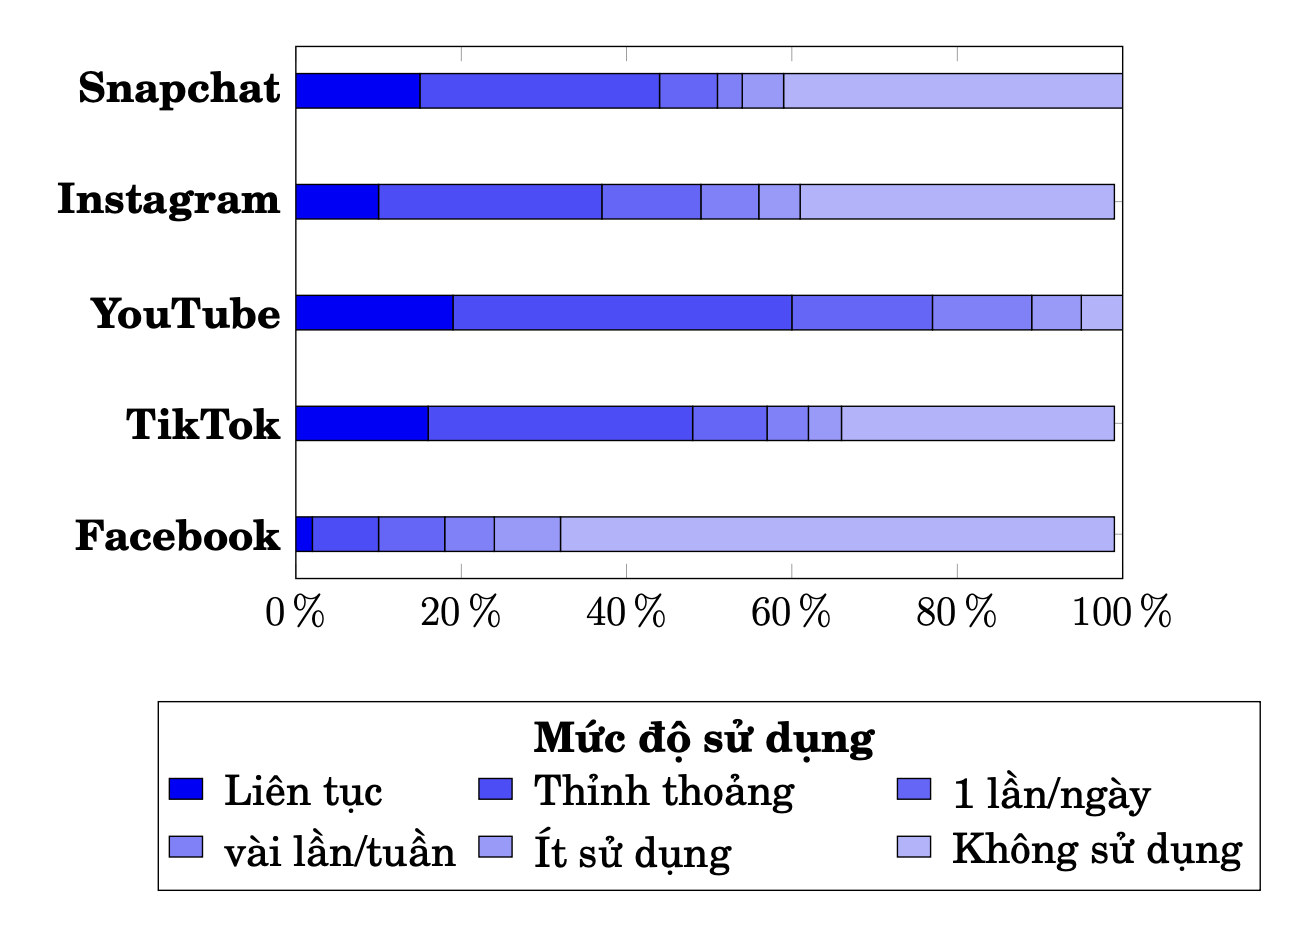
\includegraphics[width=0.8\linewidth]{/Users/chibangnguyen/Documents/GitHub/NCKH/thongkeud/trinhchieu/Screenshot 2023-11-10 at 07.06.53.png}
    \caption{\centering $\%$ thanh thiếu niên Hoa Kỳ nói rằng họ truy cập hoặc sử dụng từng trang web hoặc ứng dụng trên.}
\end{figure}    
\end{frame}

\begin{frame}
    \begin{itemize}
    \item Theo Risa Gelles-Watnick (một nhà phân tích nghiên cứu tập trung vào nghiên cứu internet và công nghệ tại Trung tâm Nghiên cứu Pew)
    \item Một số thanh thiếu niên báo cáo sử dụng các nền tảng này gần như liên tục.
    \begin{itemize}
    \item $19\%$ nói rằng họ sử dụng YouTube gần như liên tục
    \item $16\%$ và $15\%$ nói tương tự về TikTok và Snapchat, tương ứng.
    \end{itemize}
    \end{itemize}
    \begin{itemize}
        \item Nguồn:
        \begin{itemize}
        \item Khảo sát được thực hiện từ ngày 14 tháng 4 đến ngày 4 tháng 5 năm 2022.
        "Teens, Social Media and Technology 2022".
        \item Thanh thiếu niên đề cập đến những người từ 13 đến 17 tuổi. Những người không đưa ra câu trả lời sẽ không được hiển thị.
        \end{itemize}
        \end{itemize}        
\end{frame}

\begin{frame}{Thang đo Likert trong dịch vụ}
    \begin{itemize}
    \item Trong môi trường cạnh tranh khốc liệt của dịch vụ ngày nay, việc đáp ứng mong đợi của khách hàng trở thành quyết định quan trọng cho sự thành công doanh nghiệp. Để đo lường mức độ hài lòng của khách hàng, nhiều doanh nghiệp sử dụng thang đo Likert trong quá trình đánh giá chất lượng dịch vụ.
    \item Sự linh hoạt và chi tiết của thang đo Likert giúp đo lường ý kiến và cảm nhận, đặc biệt là trong đánh giá mức độ hài lòng của khách hàng. 
    \item Amazon, một đế chế thương mại điện tử toàn cầu, sử dụng thang đo Likert để khảo sát cảm nhận người dùng về quảng cáo hiển thị trên ứng dụng của họ.
    \end{itemize}
\end{frame}

\begin{frame}
\begin{figure}
    \centering
    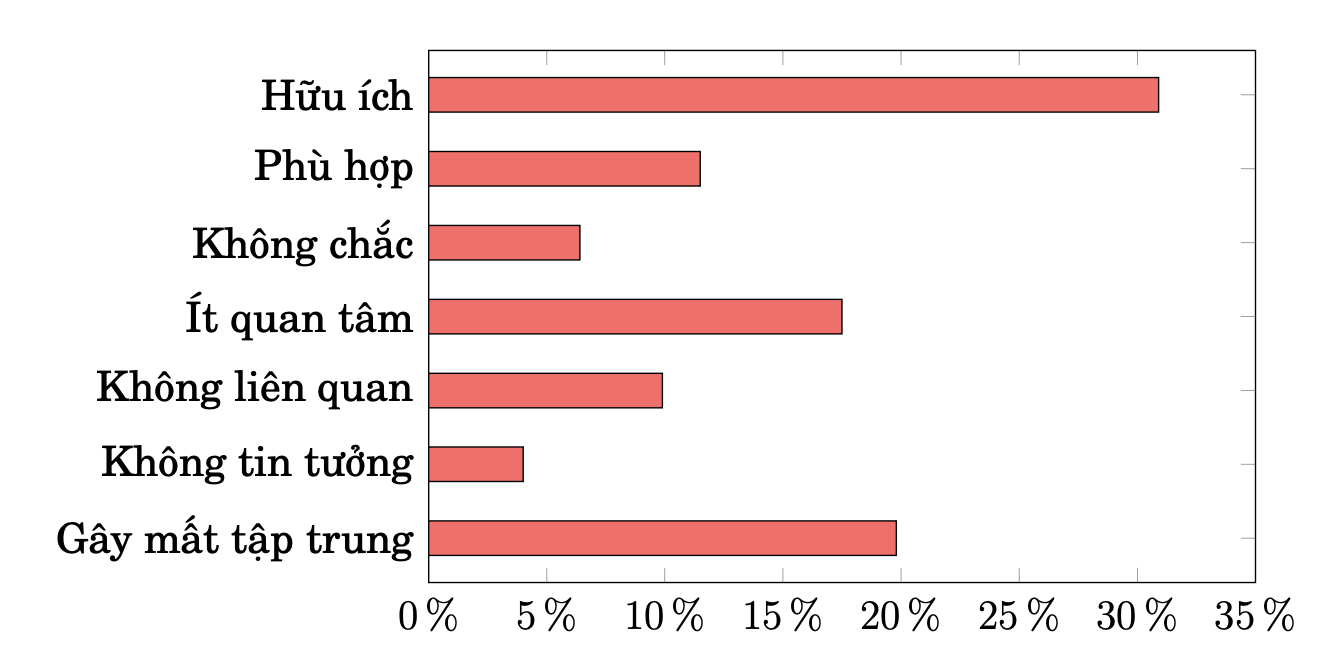
\includegraphics[width=0.9\linewidth]{/Users/chibangnguyen/Documents/GitHub/NCKH/thongkeud/trinhchieu/Screenshot 2023-11-10 at 07.07.09.png}
    \caption{\centering $\%$ người tiêu dùng cảm thấy quảng cáo được tài trợ hữu ích trên ứng dụng mua hàng Amazon.}
\end{figure}        
\end{frame}
\end{document}